% --- INSTITUTIONAL TEMPLATE FED v7.4.9 ---
% Estándar de Reporteo APA 7 (Babel-Free)
\documentclass[12pt,spanish]{article}

\usepackage{graphicx}
\usepackage{geometry}
\usepackage{indentfirst} 
\usepackage{caption}
\usepackage{floatrow} 

% Forzar estilos de caption antes de cualquier carga
\floatsetup[figure]{capposition=top}
\floatsetup[table]{capposition=top}

\usepackage{booktabs}
\usepackage{float}
\usepackage{longtable}
\usepackage{threeparttable}
\usepackage{array}
\usepackage{calc}
\usepackage{amsmath, amssymb}
\usepackage{fancyhdr}
\usepackage{mathptmx} 
\usepackage[T1]{fontenc}
\usepackage{setspace} 
\usepackage{ragged2e} 
\usepackage{titlesec}
\usepackage{url}
\def\UrlBreaks{\do\/\do-\do\.\do\_\do\?\do\=\do\&\do\%}
\usepackage[hidelinks,breaklinks]{hyperref}
\usepackage{xcolor}
\usepackage{fancyvrb}
\usepackage{framed}

% --- Code Highlighting (Pandoc Standard) ---
\newenvironment{Shaded}{\begin{snugshade}}{\end{snugshade}}
\definecolor{shadecolor}{RGB}{248,248,248}
\newenvironment{Highlighting}{}{}
\newcommand{\VerbBar}{|}
\newcommand{\VERB}{\Verb[commandchars=\\\{\}]}
\DefineVerbatimEnvironment{Highlighting}{Verbatim}{commandchars=\\\{\}}
\newcommand{\AlertTok}[1]{\textcolor[rgb]{0.94,0.16,0.16}{#1}}
\newcommand{\AnnotationTok}[1]{\textcolor[rgb]{0.56,0.35,0.01}{\textbf{\textit{#1}}}}
\newcommand{\AttributeTok}[1]{\textcolor[rgb]{0.13,0.29,0.53}{#1}}
\newcommand{\BaseNTok}[1]{\textcolor[rgb]{0.00,0.00,0.81}{#1}}
\newcommand{\BuiltInTok}[1]{#1}
\newcommand{\CharTok}[1]{\textcolor[rgb]{0.31,0.60,0.02}{#1}}
\newcommand{\CommentTok}[1]{\textcolor[rgb]{0.56,0.35,0.01}{\textit{#1}}}
\newcommand{\CommentVarTok}[1]{\textcolor[rgb]{0.56,0.35,0.01}{\textbf{\textit{#1}}}}
\newcommand{\ConstantTok}[1]{\textcolor[rgb]{0.56,0.35,0.01}{#1}}
\newcommand{\ControlFlowTok}[1]{\textcolor[rgb]{0.13,0.29,0.53}{\textbf{#1}}}
\newcommand{\DataTypeTok}[1]{\textcolor[rgb]{0.13,0.29,0.53}{#1}}
\newcommand{\DecValTok}[1]{\textcolor[rgb]{0.00,0.00,0.81}{#1}}
\newcommand{\DocumentationTok}[1]{\textcolor[rgb]{0.56,0.35,0.01}{\textbf{\textit{#1}}}}
\newcommand{\ErrorTok}[1]{\textcolor[rgb]{0.64,0.00,0.00}{\textbf{#1}}}
\newcommand{\ExtensionTok}[1]{#1}
\newcommand{\FloatTok}[1]{\textcolor[rgb]{0.00,0.00,0.81}{#1}}
\newcommand{\FunctionTok}[1]{\textcolor[rgb]{0.13,0.29,0.53}{\textbf{#1}}}
\newcommand{\ImportTok}[1]{#1}
\newcommand{\InformationTok}[1]{\textcolor[rgb]{0.56,0.35,0.01}{\textbf{\textit{#1}}}}
\newcommand{\KeywordTok}[1]{\textcolor[rgb]{0.13,0.29,0.53}{\textbf{#1}}}
\newcommand{\NormalTok}[1]{#1}
\newcommand{\OperatorTok}[1]{\textcolor[rgb]{0.81,0.36,0.00}{\textbf{#1}}}
\newcommand{\OtherTok}[1]{\textcolor[rgb]{0.56,0.35,0.01}{#1}}
\newcommand{\PreprocessorTok}[1]{\textcolor[rgb]{0.56,0.35,0.01}{\textit{#1}}}
\newcommand{\RegionMarkerTok}[1]{#1}
\newcommand{\SpecialCharTok}[1]{\textcolor[rgb]{0.81,0.36,0.00}{\textbf{#1}}}
\newcommand{\SpecialStringTok}[1]{\textcolor[rgb]{0.31,0.60,0.02}{#1}}
\newcommand{\StringTok}[1]{\textcolor[rgb]{0.31,0.60,0.02}{#1}}
\newcommand{\VariableTok}[1]{\textcolor[rgb]{0.00,0.00,0.00}{#1}}
\newcommand{\VerbatimStringTok}[1]{\textcolor[rgb]{0.31,0.60,0.02}{#1}}
\newcommand{\WarningTok}[1]{\textcolor[rgb]{0.56,0.35,0.01}{\textbf{\textit{#1}}}}

% --- Pandoc Compatibility Block (Iron Clad) ---
\providecommand{\tightlist}{%
  \setlength{\itemsep}{0pt}\setlength{\parskip}{0pt}}

% Compatibilidad Pandoc 3.x
\ifdefined\pandocbounded\else
  \newcommand{\pandocbounded}[1]{#1}
\fi

% --- Pandoc Citeproc (CSL) compatibility ---
\newlength{\cslhangindent}
\setlength{\cslhangindent}{1.27cm} 
\newlength{\csllabelwidth}
\setlength{\csllabelwidth}{3em}
\newcommand{\citeproctext}{} 
\newcommand{\citeprocitem}[2]{\item} 
\newenvironment{CSLReferences}[2] 
 {\begin{list}{}{
  \setlength{\leftmargin}{\cslhangindent}
  \setlength{\parsep}{0pt}
  \setlength{\itemsep}{6pt}
  \ifodd #1
   \setlength{\leftmargin}{\leftmargin + \csllabelwidth}
   \setlength{\itemindent}{-\csllabelwidth}
  \fi
  }
  \renewcommand{\bibitem}[2][]{\item} % Elimina los corchetes [ ]
 }
 {\end{list}}
\newcommand{\CSLBlock}[1]{#1\hfill\break}
\newcommand{\CSLLeftMargin}[1]{\parbox[t]{\csllabelwidth}{#1}}
\newcommand{\CSLRightInline}[1]{\parbox[t]{\linewidth - \csllabelwidth}{#1}\break}
\newcommand{\CSLIndent}[1]{\hspace{\cslhangindent}#1}

\makeatletter
\@ifundefined{paragraph}{\newcounter{paragraph}}{}
\@ifundefined{subparagraph}{\newcounter{subparagraph}}{}
\makeatother

% Solución al error 'No counter none defined' en longtable
\makeatletter
\newcounter{none}
\@ifpackageloaded{caption}{
  \DeclareCaptionType{none}
  \captionsetup[none]{name=Tabla}
}{}
\makeatother

\hypersetup{
  colorlinks=true,
  linkcolor=blue,
  filecolor=blue,
  citecolor=blue,
  urlcolor=blue
}

% --- Macros Institucionales ---
\newcommand{\fuente}[1]{
  \vspace{4pt}
  \begin{flushleft}
    \small
    \textit{Nota.} #1
  \end{flushleft}
}

% --- Localización Manual Determinista (Sin Babel) ---
\AtBeginDocument{
  \renewcommand{\tablename}{Tabla}
  \renewcommand{\figurename}{Figura}
  \renewcommand{\contentsname}{Índice}
  \renewcommand{\listtablename}{Índice de Tablas}
  \renewcommand{\listfigurename}{Índice de Figuras}
  \renewcommand{\abstractname}{Resumen}
  \renewcommand{\refname}{Referencias}
  
  \RaggedRight
  \setlength{\parindent}{1.27cm}
  \setlength{\parskip}{0pt}
}

\DeclareCaptionLabelSeparator{newline}{\\ \vspace{2pt}}
\captionsetup{
  position=top,
  justification=RaggedRight,
  singlelinecheck=false,
  labelfont=bf,
  textfont=it,
  labelsep=newline,
  font=small,
  skip=10pt
}
\captionsetup[figure]{name=Figura}
\captionsetup[table]{name=Tabla}

% Márgenes APA 7
\geometry{
  a4paper,
  margin=25.4mm,
  headheight=15mm
}

% --- Encabezados ---
\pagestyle{fancy}
\fancyhf{} 
\fancyhead[L]{
\includegraphics[height=1.2cm]{/home/erick-fcs/Capital_Workstation/capital-workstation-libs/src/ecs_quantitative/reporting/assets/logos/logo_unl.png}}
\fancyhead[R]{
\includegraphics[height=1.2cm]{/home/erick-fcs/Capital_Workstation/capital-workstation-libs/src/ecs_quantitative/reporting/assets/logos/logo_economia.jpg}}
\renewcommand{\headrulewidth}{0pt}
\fancyfoot[R]{\thepage}

\fancypagestyle{plain}{
  \fancyhf{}
  \fancyhead[L]{
\includegraphics[height=1.2cm]{/home/erick-fcs/Capital_Workstation/capital-workstation-libs/src/ecs_quantitative/reporting/assets/logos/logo_unl.png}}
  \fancyhead[R]{
\includegraphics[height=1.2cm]{/home/erick-fcs/Capital_Workstation/capital-workstation-libs/src/ecs_quantitative/reporting/assets/logos/logo_economia.jpg}}
  \fancyfoot[R]{\thepage}
  \renewcommand{\headrulewidth}{0pt}
}

% --- Títulos ---
\titleformat{\section}{\normalfont\normalsize\bfseries\centering}{\thesection}{1em}{}
\titleformat{\subsection}{\normalfont\normalsize\bfseries}{\thesubsection}{1em}{}
\titleformat{\subsubsection}{\normalfont\normalsize\bfseries\itshape}{\thesubsubsection}{1em}{}
\titlespacing*{\section}{0pt}{12pt}{6pt}
\titlespacing*{\subsection}{0pt}{12pt}{6pt}
\titlespacing*{\subsubsection}{0pt}{12pt}{6pt}

\newenvironment{referenciasAPA}{
  \setlength{\parindent}{-1.27cm}
  \setlength{\leftskip}{1.27cm}
  \setlength{\parskip}{6pt}
}{\par}

\begin{document}

\begin{center}
    {\bfseries \Large Universidad Nacional de Loja}\\[0.3cm]
    {\bfseries \large Facultad Jurídica, Social y
Administrativa}\\[0.2cm]
    {\bfseries Carrera de Economía}\\[1.5cm]
    
    {\bfseries \large Econometría Aplicada}\\[1cm]
    
    {\bfseries \Large ACD1: Evaluación de Impacto --- Bono de Desarrollo
Humano (BDH)}\\[1.5cm]
\end{center}

\noindent {\bfseries Estudiante:} Erick Fabricio Condoy Seraquive \\
\noindent {\bfseries Docente:} Eco. José Rafael Alvarado López \\
\noindent {\bfseries Fecha:} 20 de abril de 2026 \\

\vspace{1cm}

\doublespacing
\setlength{\parindent}{1.27cm}

\section{Introducción}\label{introducciuxf3n}

La evaluación de impacto de las políticas sociales es fundamental para
determinar si los recursos públicos están cumpliendo sus objetivos de
bienestar sin generar distorsiones negativas en el mercado laboral. En
esta entrega, se analiza el \textbf{Bono de Desarrollo Humano (BDH)},
una transferencia monetaria condicionada dirigida a los hogares en
situación de vulnerabilidad extrema en Ecuador (MIES 2024). El objetivo
central es identificar si la recepción de este subsidio correlaciona con
la probabilidad de desempeñarse en el \textbf{sector informal}.

\section{Descripción de Variables}\label{descripciuxf3n-de-variables}

Para la estimación del modelo de impacto, se han seleccionado variables
sociodemográficas y de control económico extraídas y depuradas de la
ENEMDU 2023-2024 (INEC 2024), filtrando a la Población Económicamente
Activa (PEA) de entre 15 y 65 años.

\begin{longtable}[]{@{}
  >{\raggedright\arraybackslash}p{(\linewidth - 6\tabcolsep) * \real{0.2500}}
  >{\raggedright\arraybackslash}p{(\linewidth - 6\tabcolsep) * \real{0.2500}}
  >{\raggedright\arraybackslash}p{(\linewidth - 6\tabcolsep) * \real{0.2500}}
  >{\raggedright\arraybackslash}p{(\linewidth - 6\tabcolsep) * \real{0.2500}}@{}}
\caption{Variables del Modelo de Evaluación de
Impacto}\label{tbl-variables}\tabularnewline
\toprule\noalign{}
\begin{minipage}[b]{\linewidth}\raggedright
Variable
\end{minipage} & \begin{minipage}[b]{\linewidth}\raggedright
Tipo
\end{minipage} & \begin{minipage}[b]{\linewidth}\raggedright
Descripción
\end{minipage} & \begin{minipage}[b]{\linewidth}\raggedright
Fuente
\end{minipage} \\
\midrule\noalign{}
\endfirsthead
\toprule\noalign{}
\begin{minipage}[b]{\linewidth}\raggedright
Variable
\end{minipage} & \begin{minipage}[b]{\linewidth}\raggedright
Tipo
\end{minipage} & \begin{minipage}[b]{\linewidth}\raggedright
Descripción
\end{minipage} & \begin{minipage}[b]{\linewidth}\raggedright
Fuente
\end{minipage} \\
\midrule\noalign{}
\endhead
\bottomrule\noalign{}
\endlastfoot
\texttt{age} & Entero & Edad cronológica del encuestado (15-65 años) &
ENEMDU \\
\texttt{sex} & Binaria & Género (1: Hombre; 0: Mujer) & ENEMDU \\
\texttt{edu} & Categórica & Nivel de instrucción formal alcanzado &
ENEMDU \\
\texttt{hh\_size} & Entero & Número de miembros que integran el hogar &
ENEMDU \\
\texttt{area} & Binaria & Ubicación geográfica (1: Urbana; 0: Rural) &
ENEMDU \\
\texttt{treated} & Binaria & Receptor del Bono de Desarrollo Humano
(Tratamiento) & ENEMDU \\
\texttt{informal} & Binaria & Pertenencia al sector informal (Variable
de Resultado) & Construcción Propia \\
\end{longtable}

\section{Metodología}\label{metodologuxeda}

Debido a que el BDH no se asigna de forma aleatoria, se emplea el modelo
de \textbf{Propensity Score Matching (PSM)} para corregir el sesgo de
selección (Shmueli 2010). Se estima el \emph{Propensity Score} mediante
un modelo Logit, controlando por las variables descritas en la
Table~\ref{tbl-variables}. El emparejamiento se realiza mediante el
algoritmo de \textbf{Vecino más Cercano (1:1)} con un \emph{caliper} de
\(0.25\sigma\).

\section{Resultados}\label{resultados}

\subsection{Efecto Medio del Tratamiento
(ATT)}\label{efecto-medio-del-tratamiento-att}

Tras el matching, se obtuvo un \textbf{ATT (Average Treatment Effect on
the Treated)} de \textbf{+39.32\%}. Esto indica que los beneficiarios
del BDH tienen una probabilidad significativamente mayor de trabajar en
la informalidad que el grupo de control comparable.

\subsection{Soporte Común y Balance}\label{soporte-comuxfan-y-balance}

En la Figure~\ref{fig-pscore} se presenta la distribución del P-Score,
confirmando un soporte común adecuado. Asimismo, la
Figure~\ref{fig-balance} muestra el balance de la variable edad tras el
emparejamiento.

\begin{figure}

\centering{

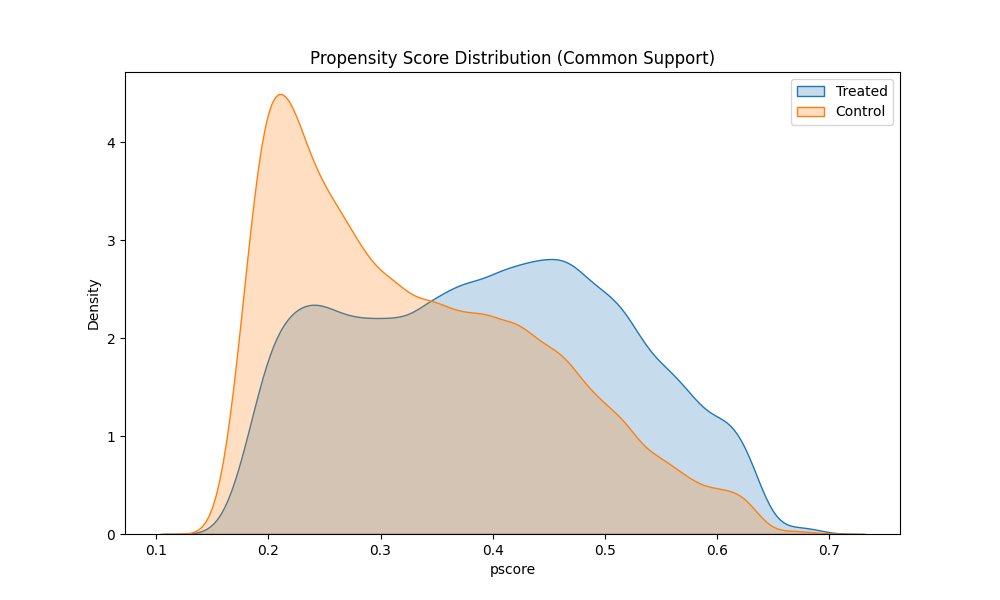
\includegraphics[width=0.75\linewidth,height=\textheight,keepaspectratio]{plots/common_support_bdh.png}

}

\caption{\label{fig-pscore}Distribución de Propensity Score (Soporte
Común)}

\end{figure}%

\begin{figure}

\centering{

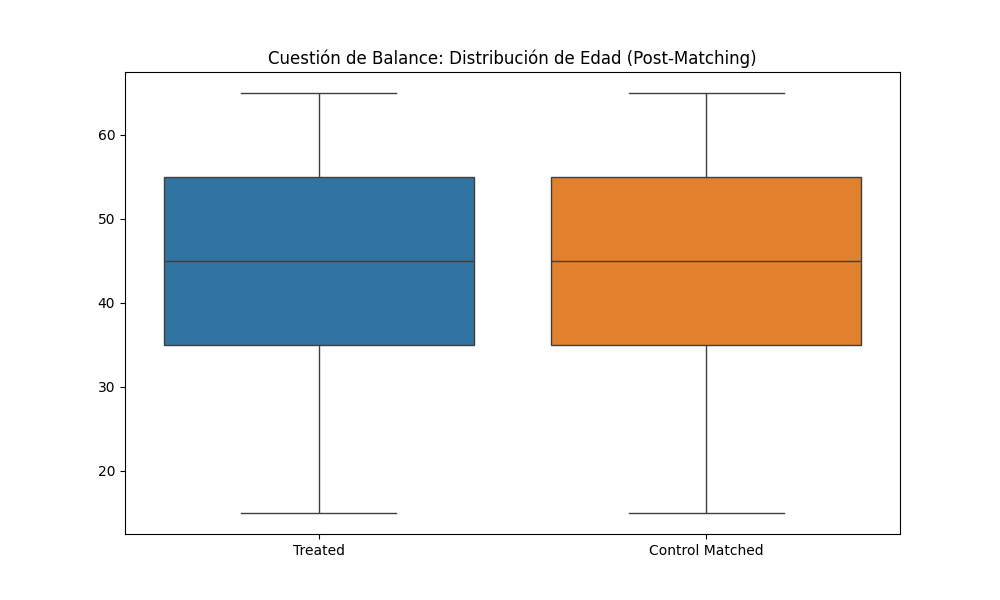
\includegraphics[width=0.75\linewidth,height=\textheight,keepaspectratio]{plots/age_balance_post.png}

}

\caption{\label{fig-balance}Balance de Covariables: Edad Post-Matching}

\end{figure}%

\section{Conclusión}\label{conclusiuxf3n}

Los resultados sugieren que el BDH puede estar actuando como un
desincentivo a la formalización laboral en el margen de la pobreza
extrema, fenómeno conocido como la ``Trampa de Informalidad''. Se
recomienda una revisión de las condicionalidades del programa para
fomentar la transición hacia empleos de mayor productividad.

\section{Referencias}\label{referencias}

\protect\phantomsection\label{refs}
\begin{CSLReferences}{1}{1}
\bibitem[\citeproctext]{ref-enemdu2024}
INEC. 2024. \emph{Encuesta Nacional de Empleo, Desempleo y Subempleo
(ENEMDU): Metodología de Cálculo de La Informalidad}. Instituto Nacional
de Estadística y Censos de Ecuador.

\bibitem[\citeproctext]{ref-bdh2024}
MIES. 2024. \emph{Bono de Desarrollo Humano: Impacto En El Bienestar y
Mercado Laboral}. Ministerio de Inclusión Económica y Social de Ecuador.

\bibitem[\citeproctext]{ref-shmueli2010}
Shmueli, Galit. 2010. {``To Explain or to Predict?''} \emph{Statistical
Science} 25 (3): 289--310.

\end{CSLReferences}

\end{document}
